\section*{VAE's}
\begin{frame}{Variational Autoencoder (VAE)}
    \begin{figure}
        \centering
        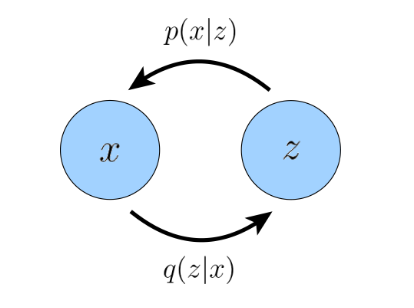
\includegraphics[width=0.4\textwidth]{Images/vae1.png}
        \caption{Variational Autoencoder}
    \end{figure}

    In default formulation in VAE paper, directly maximize ELBO using a \textcolor{blue}{variational} approach. \\

    We optimize for best possible $q_{\phi}(z|x)$ among family of posterior distributions which are parameterized by $\phi$.

\end{frame} 

\begin{frame}{Family of Posterior Distributions}
    The family of posterior distributions is generally choosen as multivariate gaussian with diagonal covariance matrix.

    \begin{align*}
        q_{\phi}(z|x) &= \mathcal{N}(z ; \mu_{\phi}(x), \sigma_{\phi}(x)) \\
        &= \mathcal{N}(z;\mu_{\phi}(x), diag(\sigma_{\phi}(x)))
    \end{align*}

    The prior is choosen as standard normal distribution 
    \begin{align*}
        p(z) &= \mathcal{N}(z;0, \mathbb{I}_{d \times d})
    \end{align*}
\end{frame}

\begin{frame}{Encoder and Decoder Network}
    When we maximize the ELBO, we are doing the following things to be specific:
    \begin{enumerate}
        \item Adjusting parameters $\phi$ in such a way that true latent distribution $p(z)$ is as close as possible to encoder outputs $p(z|x)$.
        \item Using these latents to regenerate the true data $x$ as close as possible.
    \end{enumerate}

    Let us see what they mean
\end{frame}

\begin{frame}{ELBO again}
    \begin{align*}
        ELBO &= \mathbb{E}_{q(z|x)}[log\left(\frac{p(x,z)}{q(z|x)}\right)] \\
        &= \mathbb{E}_{q(z|x)}[log \left( \frac{p(z)p(x | z)}{q(z|x)} \right)] \\
        &= \mathbb{E}_{q(z|x)}[log(p(x|z)) + log\left(\frac{p(z)}{q(z|x)}\right)] \\
        &= \mathbb{E}_{q(z|x)}[log(p(x|z))] + \mathbb{E}_{q(z|x)}[log\left(\frac{p(z)}{q(z|x)}\right)] \\
        &= \mathbb{E}_{q(z|x)}[log(p(x|z))] - \mathbb{E}_{q(z|x)}[log\left(\frac{q(z|x)}{p(z)}\right)] \\
        &= \mathbb{E}_{q(z|x)}[log(p(x|z))] - KL(q(z|x) || p(z))
    \end{align*}
\end{frame}

\begin{frame}{Continued}
    While maximizing ELBO, we did 2 things:
    \begin{enumerate}
        \item Maximize $\mathbb{E}_{q(z|x)}[log(p(x|z))]$ - This is the reconstruction term.
        \item Minimize $KL(q(z|x) || p(z))$ - This is the prior matching term.
    \end{enumerate}

    \bigskip

    Look at 2nd term first, this tries to bring $q(z|x)$ close to $p(z)$, which means given $x$, we are trying to model $z$ as close as possible to true latent distribution. 

    \bigskip

    Now look at 1st term in which we maximize the log likelihood of generating back the true $x$ from $z$. 
\end{frame}

\begin{frame}{Computing ELBO}
    There are 2 terms to be computed in ELBO:
    \begin{enumerate}
        \item Reconstruction term: $\mathbb{E}_{q(z|x)}[log(p(x|z))]$
    \end{enumerate}

    This can be estimated using sample averages. We sample $\{z^{(i)}\}_{i=1}^{N} \sim q(z|x)$  then above term can be computed as 
    \begin{align*}
        \mathbb{E}_{q(z|x)}[log(p(x|z))] &= \frac{1}{N} \sum_{i=1}^{N} log(p(x|z^{(i)}))
    \end{align*}
\end{frame}

\begin{frame}{Computing ELBO}
    \begin{enumerate}
        \setcounter{enumi}{1}
        \item KL Divergence term: $KL(q(z|x) || p(z))$
    \end{enumerate}
    Since both $q(z|x)$ and $p(z)$ are gaussian, there exists a closed form solution to compute KL divergence between 2 gaussians.
\end{frame}

